\section{Experiment}

\subsection{Setup}

In our study, we constructed a simulation framework consisting of two networks:
an honest party network comprising 37 nodes and an adversarial network with 12
nodes. The honest party had an artificial network delay of 100ms and
expected block production time was set to 1 second. Adversaries network delay
was only the inherent delay in communication between virtual machines and was
<5 ms. This configuration establishes the adversary's hash rate, denoted as
$\beta$, at 24.44 for our experiments. PoEM experiments were run utilizing a
bias factor of 14.6. Our primary objective is to measure the confirmation delay
(denoted as $d$) under varying block rates ($g$) for both PoEM and Bitcoin
protocols.

For each experimental setup, we fixed the value of gg and conducted a Monte
Carlo simulation comprising 100 iterations. In each iteration, we determined
the winner of each round by identifying which party reached that round quickest
from the experiment's onset. Upon completing 100 iterations, we aggregated the
victories of the honest party for each run. We then calculated the frequency
($f$) at which the probability of the honest parties' victory surpasses 90\%.
The confirmation delay ($d$) for each experiment was obtained by dividing $f$
by $g$.

Figure 1 illustrates the evolution of $d$ across different $g$ values. We
identified the best operating conditions for a protocol as the point where the
confirmation delay is minimized. In our simulations, Bitcoin achieved its
lowest delay of 11.16 at a block rate of $g=0.98$. Conversely, PoEM reached its
minimal delay of 10.58 at a higher block rate of $g=1.29$, indicating that PoEM
can operate at a 31.6\% faster rate while still attaining a lower confirmation
delay compared to Bitcoin.

Further, we extended our simulation to examine PoEM's performance with varied
bias values, specifically at Bitcoin's optimal operating point of $g=0.98$.
Figure 2 presents the confirmation delays corresponding to different bias
values. These results demonstrate that PoEM can achieve even lower confirmation
delays with optimized $\gamma$ values. Notably, the optimal confirmation delay
of 7.95 was observed at a bias setting of 10. However, the optimization of
$\gamma$ for all values of $g$ is a non-trivial task, and we leave this to
future work.

\begin{figure}
    \centering
    \begin{subfigure}{0.49\textwidth}
    \centering
    \caption{d vs g}
    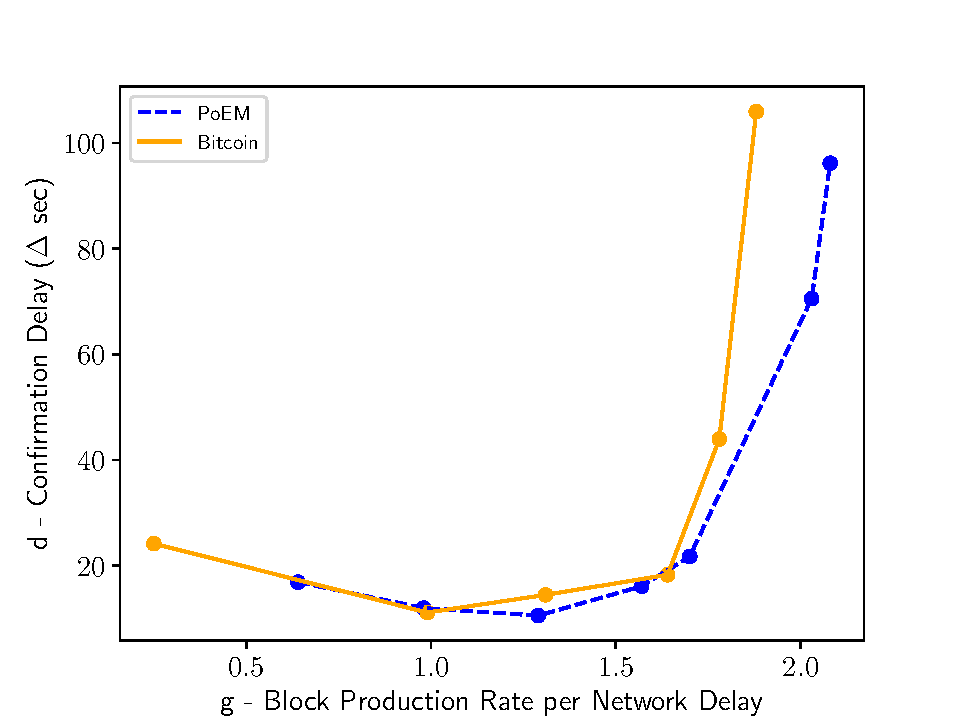
\includegraphics[width = 0.8\textwidth]{figures/dvsg.pdf}
    \label{fig:dvsg}
    \end{subfigure}
    \begin{subfigure}{0.49\textwidth}
    \centering
    \caption{d vs bias}
    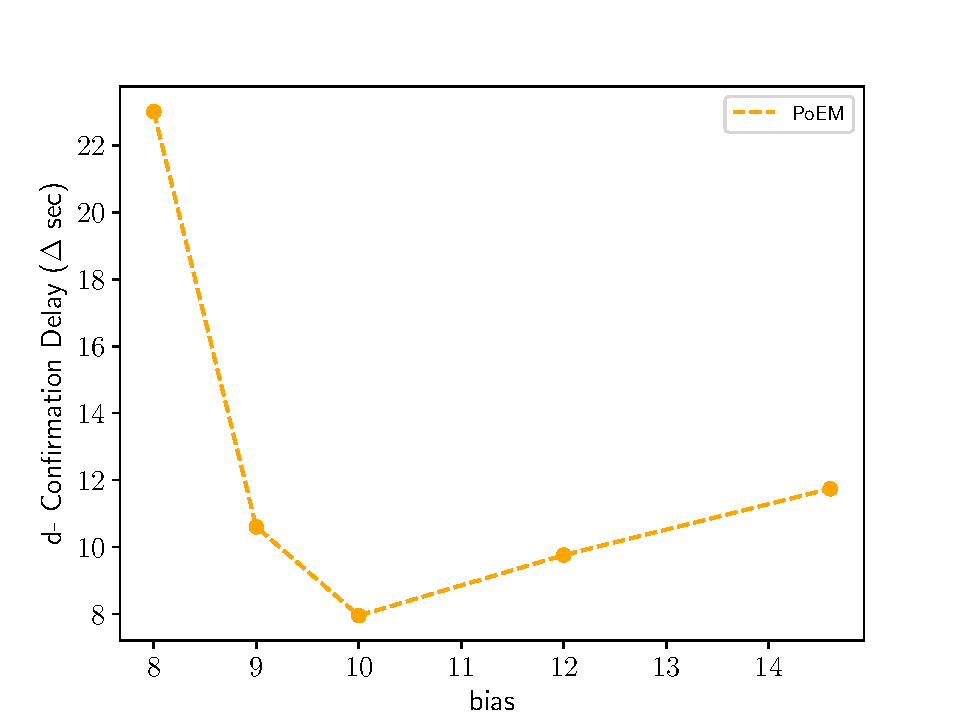
\includegraphics[width = 0.8\textwidth]{figures/gamma.pdf}
    \label{fig:right}
    \end{subfigure}
    \caption{Confirmation delay from simulations of PoEM and Bitcoin for various values of $g$ a) Confirmation delay $\Delta$ vs. the block production rate $g$. Note that PoEM typically demonstrates lower confirmation delay for any given value of $g$, and the difference becomes more pronounced at large $g$ b) Confirmation delay ($\Delta$) vs. the bias $\gamma$. The bias, $\gamma$ was experimentally optimized for the $g$ which showed the lowest confirmation delay in Bitcoin to elucidate the optimized performance of PoEM. PoEM achieved confirmation 28.8\% faster than Bitcoin's most optimal performance.}
    \label{fig:gamma}
\end{figure}

\subsection{Practical Deployment}
PoEM consensus mechanism has been deployed in real world as a consensus
mechanism for the Quai Networks Iron Age Testnet. The testnet was started in
October 2023 and has been running since. As of 24th Jan 2024, over 7.5 million
blocks have been mined with over 2000 Miners, Node operators participating in
the testnet and over 500 million transactions have been confirmed in the network
using the consensus mechanism. The network has maintained an average hash rate
of over 50GH/s during this time period.
